\documentclass[10pt]{beamer}
\usepackage[utf8]{inputenc}
\usepackage{textpos}
\usepackage{tikz}
\usepackage{grid-system}
\usepackage{currfile}
\usepackage{color}
\usepackage{enumitem}
\usepackage[T1]{fontenc}
\usepackage[sfdefault]{AlegreyaSans}

\usetheme{default}
\usecolortheme{dove}

\definecolor{freifunkpink}{RGB}{215,0,73}
\definecolor{freifunkyellow}{RGB}{255,191,0}
\definecolor{lightgrey}{RGB}{220,220,220}

\setlist[itemize]{leftmargin=*}

\renewcommand*\oldstylenums[1]{{\AlegreyaSansOsF #1}}

\AtBeginSection[]
{
  \begin{frame}<beamer>
    \frametitle{Übersicht}
    \tableofcontents[currentsection]
  \end{frame}
}

\usebackgroundtemplate%
{%
    \tikz[overlay,remember picture]
    \node[opacity=0.26, at=(current page.south east),anchor=south east,inner sep=0pt] {
        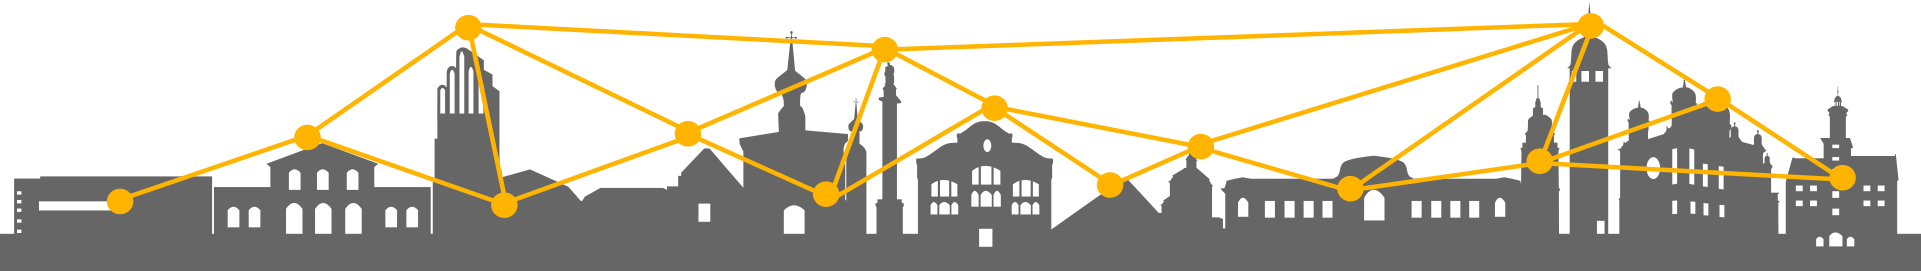
\includegraphics[width=\paperwidth]{images/footer_dark}
    };
}

  \addtobeamertemplate{frametitle}{}{
    \begin{textblock*}{0cm}(\textwidth-0.85cm,-0.85cm)
      \begin{figure}[h]
        \def\svgwidth{1.5cm}
        \input{logo.pdf_tex}
      \end{figure}
    \end{textblock*}
  }

\title{Freifunk Ortenau}
\author{}
\date{\footnotesize 30. Juli 2016}

\begin{document}

{
  \usebackgroundtemplate{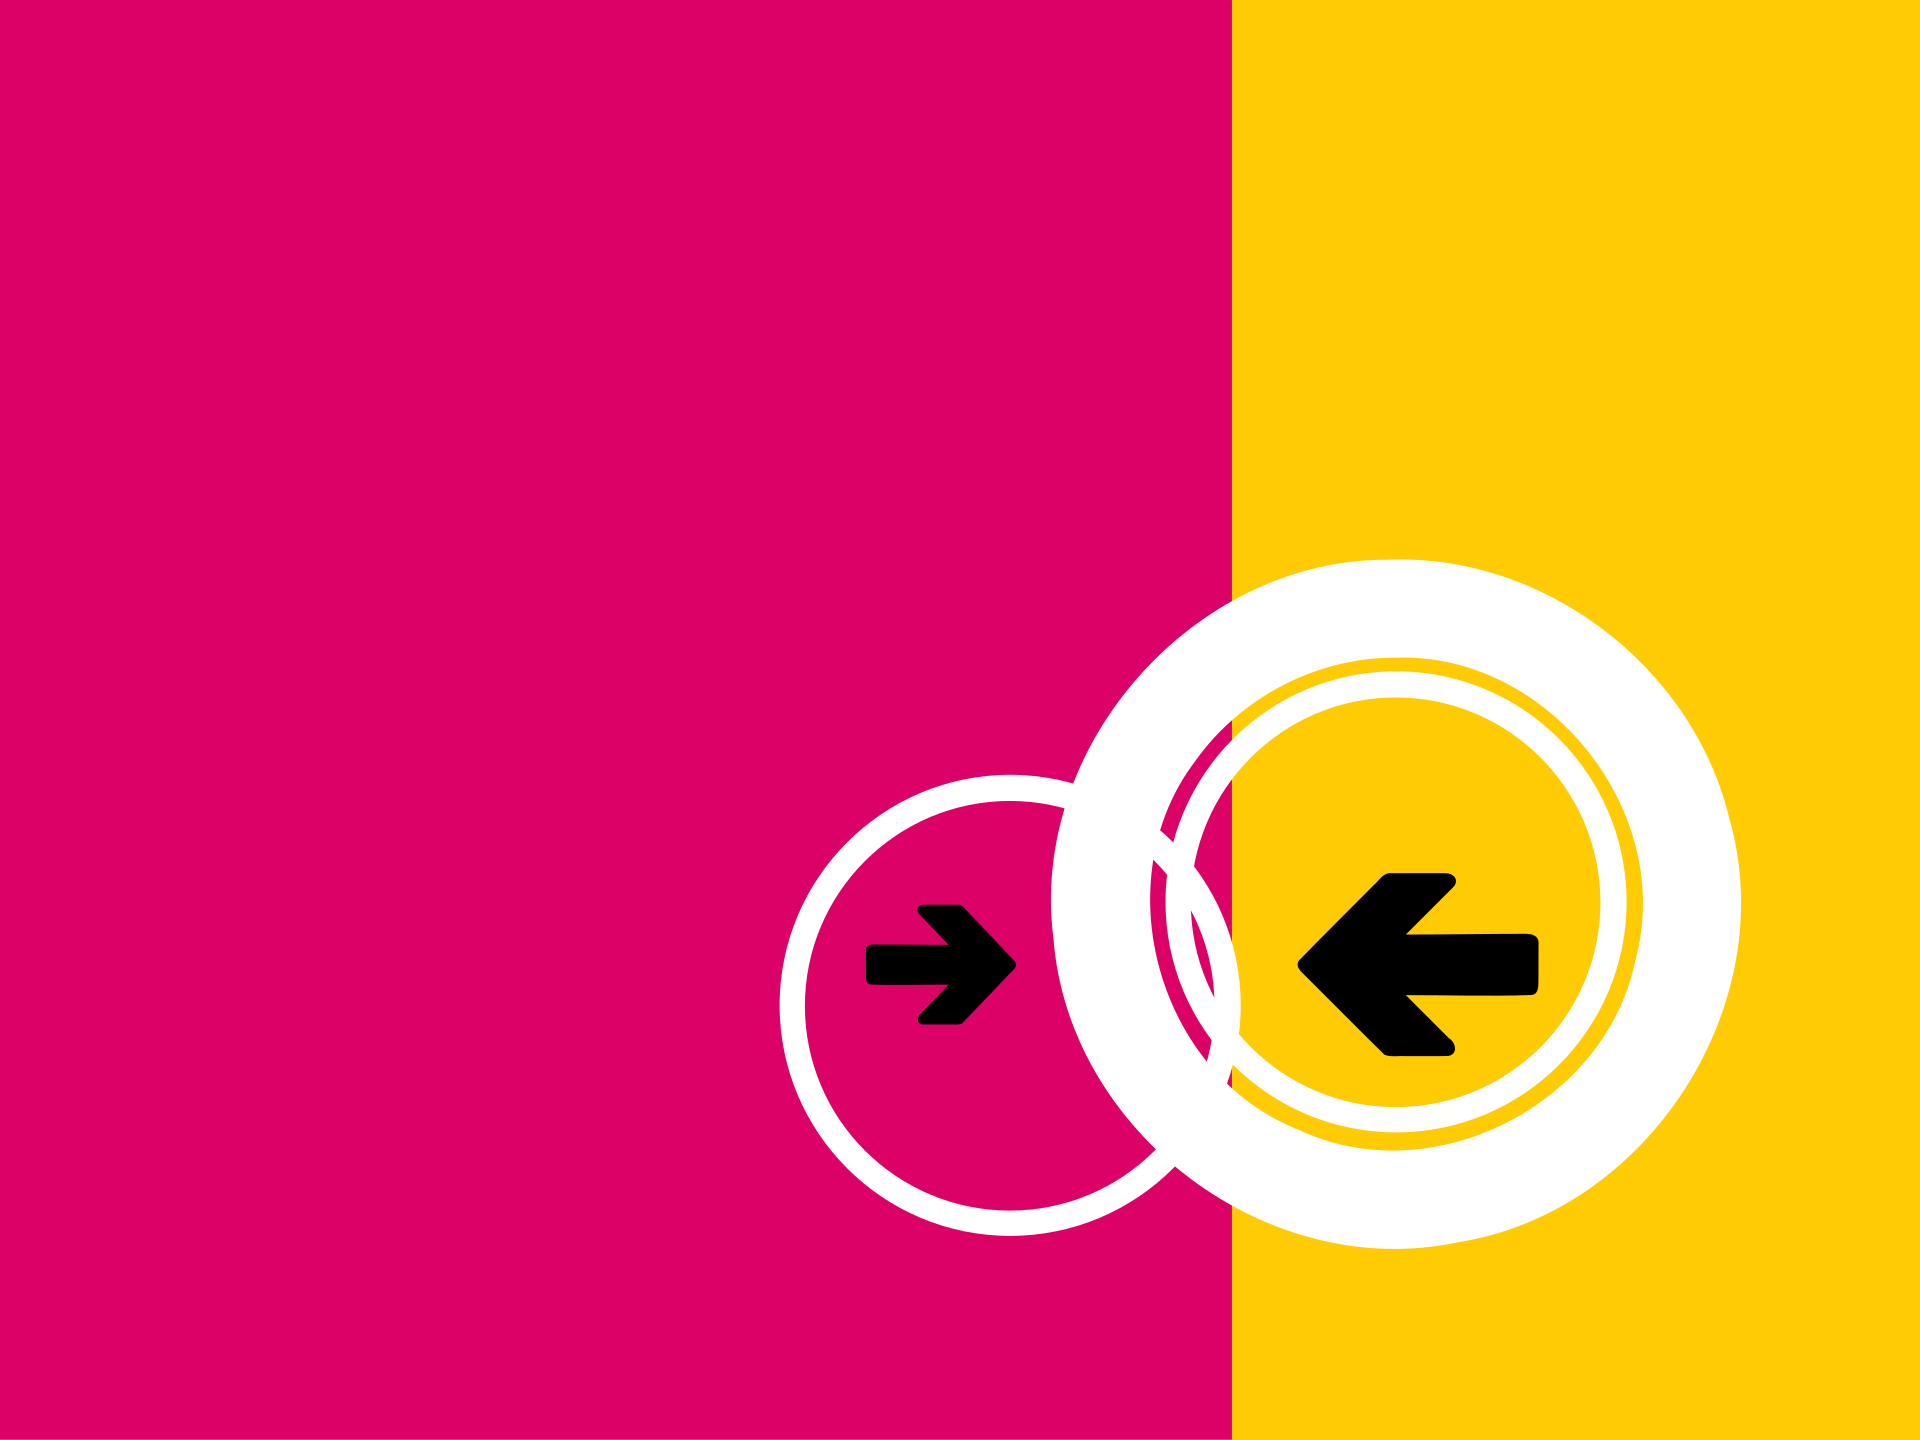
\includegraphics[width=\paperwidth]{images/logo_magenta_yellow.png}}
  \begin{frame}
    \begin{huge}
      Freifunk Ortenau
    \end{huge}
    \vspace{0.25em}
    \newline
    Das freie und gemeinschaftliche Netz
    \newline
    \vspace{0.5em}
    \newline
    \small{30. Juli 2016}
    \vfill
  \end{frame}
}

  \section{Was ist Freifunk}

  \begin{frame}{Was ist Freifunk?}
      \begin{center}
        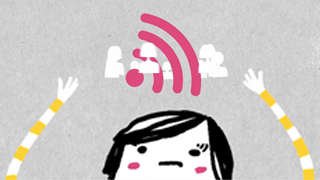
\includegraphics[width=3.6cm]{images/up}
      \end{center}
      Wie wäre es, wenn\ldots
      \begin{itemize}
        \pause
        \item[\textcolor{freifunkpink}{\Large$\bullet$}] du kostenlos, einfach und anonym ein WLAN nutzen könntest, \textbf{ohne eine Firma}, bei der man sich registrieren muss?
        \pause
        \item[\textcolor{freifunkpink}{\Large$\bullet$}] du deinen Internetanschluss gefahrlos teilen könntest \textbf{ohne} dir um die \textbf{Störerhaftung} Gedanken machen zu müssen?
        \pause
        \item[\textcolor{freifunkpink}{\Large$\bullet$}] du ein Teil eines Netzwerkes wärst, das \textbf{frei von Zensur} ist und das man \textbf{nicht so einfach abschalten kann}.
      \end{itemize}
    \end{frame}

    \begin{frame}{Was ist Freifunk?}
      Freifunk steht für \textbf{freie Netze}, frei wird dabei verstanden als\ldots
      \begin{center}
        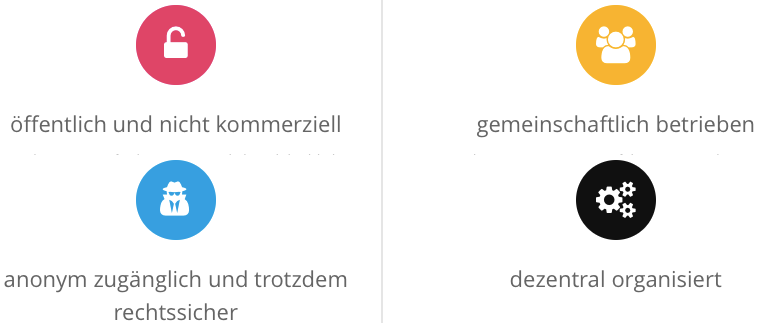
\includegraphics[width=10cm]{images/principles}\\
      \end{center}
    \end{frame}

    \begin{frame}{Was ist Freifunk?}
    \begin{columns}[T]
     \begin{column}{5cm}
        \begin{itemize}
          \item[\textcolor{freifunkpink}{\Large$\bullet$}] Über \textbf{300} regionale Freifunk Communities in Deutschland
          \item[\textcolor{freifunkpink}{\Large$\bullet$}] Betreiben bundesweit über \textbf{35.000} Zugangspunkte
          \item[\textcolor{freifunkpink}{\Large$\bullet$}] Communities unterstützen sich gegenseitig und entwickeln Freifunk-Software gemeinsam
          \item[\textcolor{freifunkpink}{\Large$\bullet$}] Austausch auf Konferenzen, Mailverteiler und Chats
        \end{itemize}
      \end{column}
      \begin{column}{5cm}
        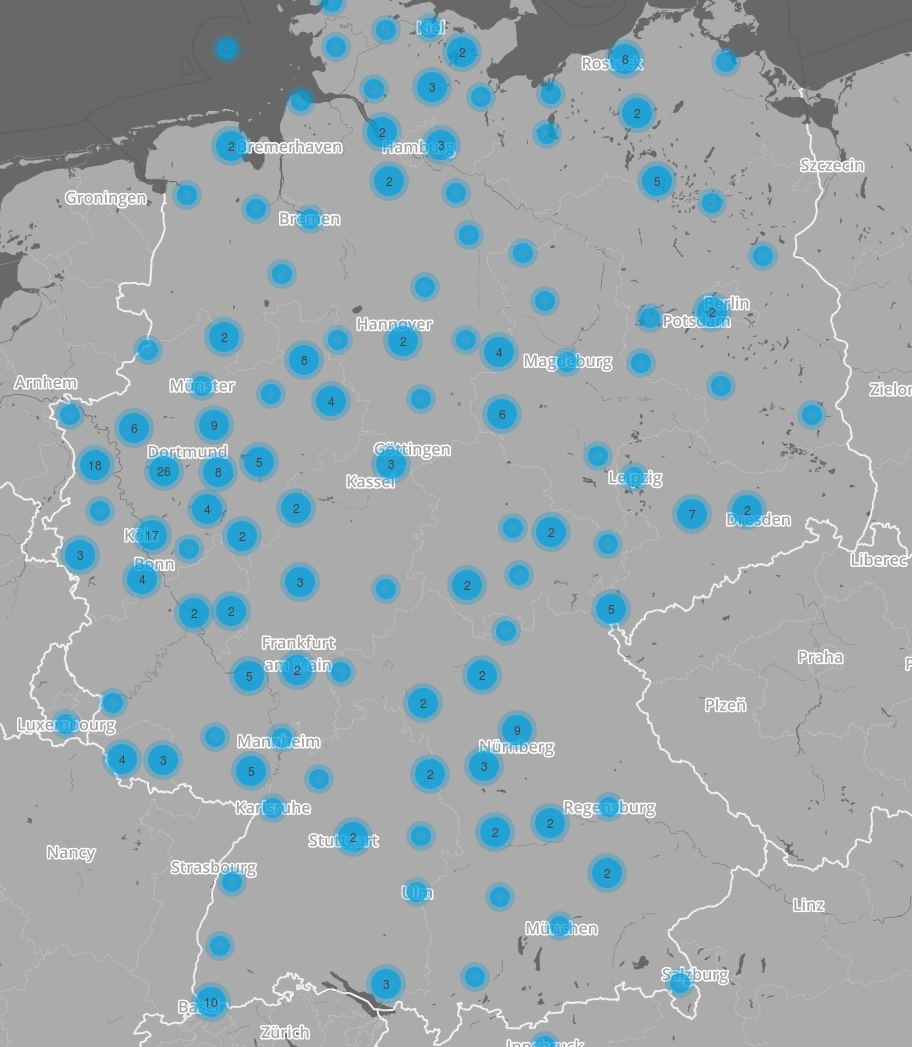
\includegraphics[width=0.9\textwidth]{images/community_map}
      \end{column}
    \end{columns}
   \end{frame}


    \begin{frame}{Was ist Freifunk?}
    \begin{columns}[T]
     \begin{column}{4cm}
	\vspace{1em}
    	
\includegraphics[width=0.9\textwidth]{images/talk}\\
      \end{column}
      \begin{column}{6cm}
        \begin{itemize}
          \item[\textcolor{freifunkpink}{\Large$\bullet$}] \textbf{Ehrenamtliche} entwickeln und errichten freie WLAN-Netzwerke
          \item[\textcolor{freifunkpink}{\Large$\bullet$}] Freifunk versteht sich \textbf{nicht als Dienstleister}, sondern als \textbf{,,Mitmachnetz''}
          \item[\textcolor{freifunkpink}{\Large$\bullet$}] Infrastruktur \textbf{finanziert} sich \textbf{durch Spenden}
          \item[\textcolor{freifunkpink}{\Large$\bullet$}] Viele Freifunk Communities bieten \textbf{Zugang zum Internet} und zwar \textbf{rechtssicher}
          \item[\textcolor{freifunkpink}{\Large$\bullet$}] Jeder kann mitmachen und das \textbf{Netz erweitern}
        \end{itemize}
      \end{column}
    \end{columns}
   \end{frame}


  \begin{frame}{Weitere Ziele von Freifunk}
    \begin{columns}[T]
     \begin{column}{5cm}
        \begin{itemize}
          \item[\textcolor{freifunkpink}{\Large$\bullet$}] \textbf{Verständnis von Kommunikationsnetzen} sowie deren Auswirkungen auf die Gesellschaft fördern
          \item[\textcolor{freifunkpink}{\Large$\bullet$}] Teilnahme der Bevölkerung an \textbf{Forschung und Aufbau} dezentraler Netze
          \item[\textcolor{freifunkpink}{\Large$\bullet$}] \textbf{Wissen und Software} öffentlich zugänglich machen
          \item[\textcolor{freifunkpink}{\Large$\bullet$}] Beteiligung an politischen Prozessen, um \textbf{rechtliche Voraussetzungen} für freie Netze zu schaffen
        \end{itemize}
      \end{column}
      \begin{column}{5cm}
        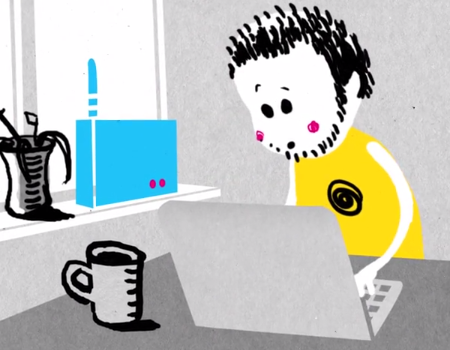
\includegraphics[width=0.9\textwidth]{images/install}
      \end{column}
    \end{columns}
  \end{frame}

  \section{Wie Freifunk funktioniert}

  \begin{frame}{Ohne Freifunk}
    \begin{center}
      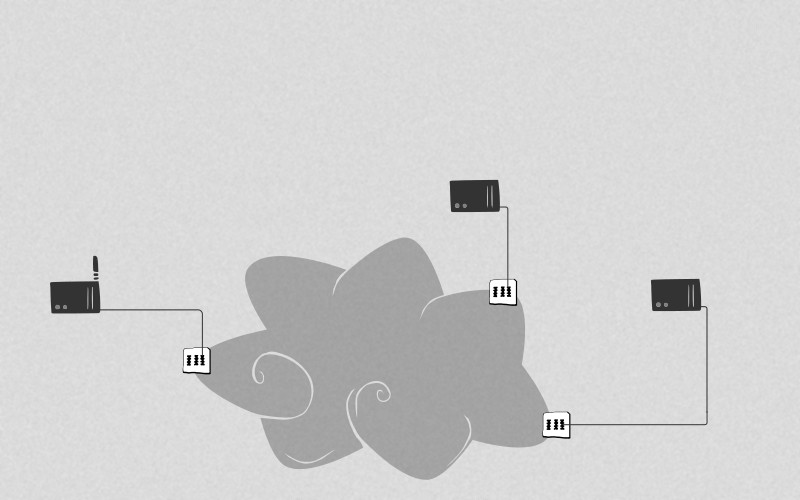
\includegraphics[height=5cm]{images/network_1}\\
      \vspace{1em}
      Geschlossene WLAN-Netze, welche nicht miteinander kommunizieren\\
      \vspace{1em}
    \end{center}
  \end{frame}

  \begin{frame}{Mit Freifunk}
    \begin{center}
      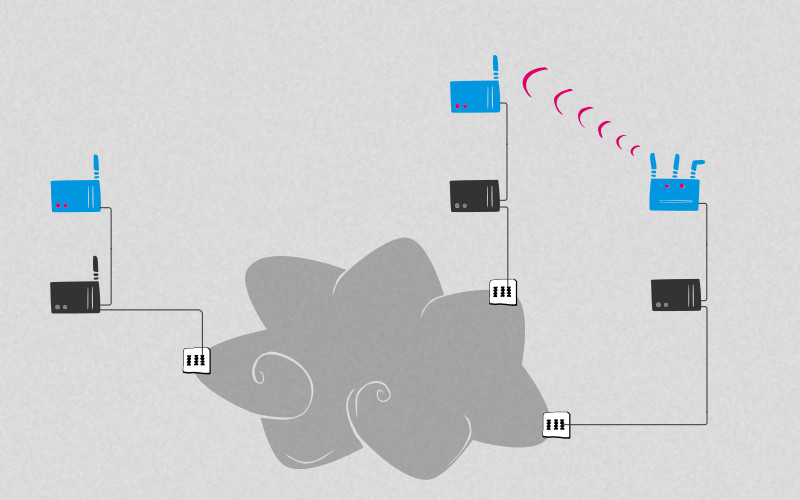
\includegraphics[height=5cm]{images/network_2}\\
      \vspace{1em}
      Dein Freifunk-Knoten bildet ein Teil des freien Netzes und verbindet sich mit anderen Knoten
    \end{center}
  \end{frame}

  \begin{frame}{Verminderung der digitalen Kluft}
    \begin{center}
      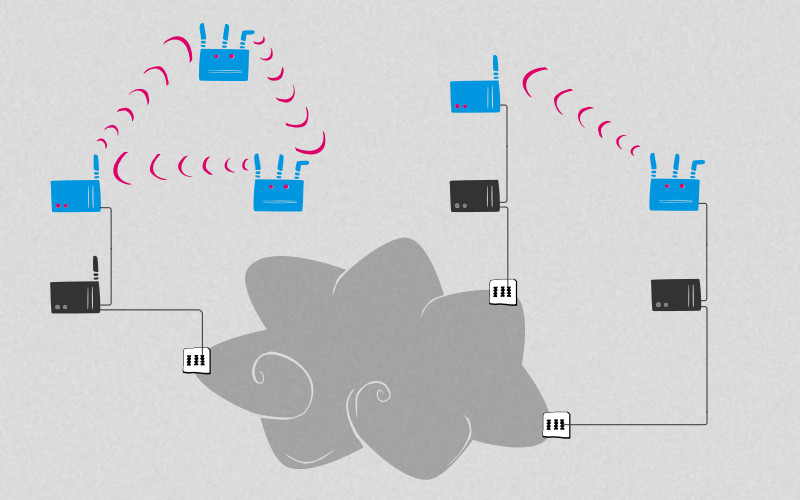
\includegraphics[height=5cm]{images/network_3}\\
      \vspace{1em}
      Neue Knoten ohne Internetzugang kommen hinzu\\
      \vspace{1em}
    \end{center}
  \end{frame}

  \begin{frame}{Das Heimnetz bleibt privat}
    \begin{center}
      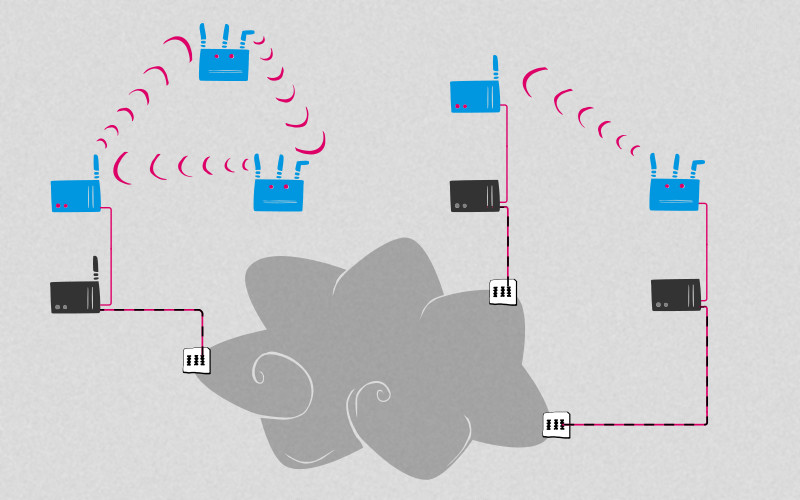
\includegraphics[height=5cm]{images/network_4}\\
      \vspace{1em}
      Dein Heimnetz bleibt vor Zugriffen über Freifunk geschützt
      \vspace{1em}
    \end{center}
  \end{frame}

  \begin{frame}{Zugang zum Internet}
    \begin{center}
      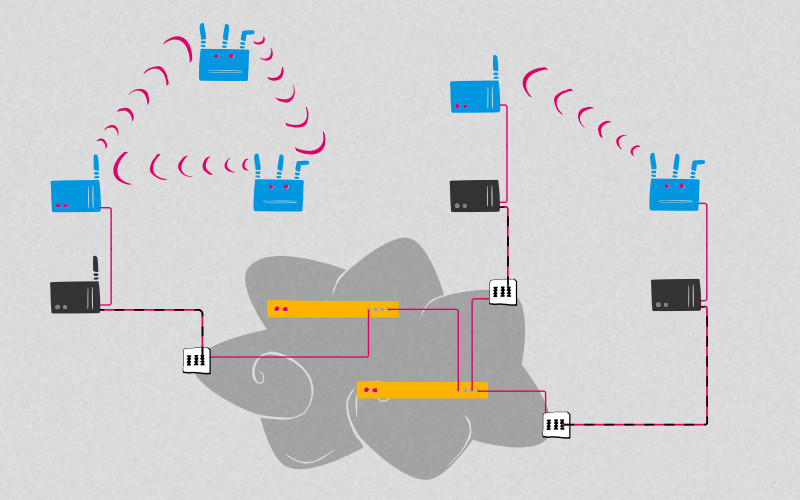
\includegraphics[height=5cm]{images/network_5}\\
      \vspace{1em}
      Freifunk Gateways verbinden Freifunk-Knoten über weite Strecken und stellen Internetverbindung bereit
    \end{center}
  \end{frame}

  \begin{frame}{Und was ist mit der Störerhaftung?}
    \begin{columns}[T]
     \begin{column}{4cm}
    	
\includegraphics[height=5cm]{images/recht}\\
      \end{column}
      \begin{column}{6cm}
        \begin{itemize}
          \item[\textcolor{freifunkpink}{\Large$\bullet$}] Am 26.07.2016 ist das \textit{Zweite Gesetz zur Änderung des Telemediengesetzes} in Kraft getreten
          \item[\textcolor{freifunkpink}{\Large$\bullet$}] Ziel war es, die Störerhaftung abzuschaffen. Juristen halten Gesetztesänderung für nicht ausreichend.
          \item[\textcolor{freifunkpink}{\Large$\bullet$}] Abmahnkanzleien haben angekündigt \textbf{weiterhin abzumahnen}.
          \item[\textcolor{freifunkpink}{\Large$\bullet$}] Eine \textbf{rechtliche unsicherheit} bleibt also \textbf{weiterhin bestehen} 
        \end{itemize}
      \end{column}
    \end{columns}
  \end{frame}

  \begin{frame}{Und was ist mit der Störerhaftung?}
    \begin{columns}[T]
     \begin{column}{5cm}
        \begin{itemize}
          \item[\textcolor{freifunkpink}{\Large$\bullet$}] Datenverkehr des Freifunk-WLANs wird über ein \textbf{verschlüsseltes VPN} zu unseren Gateways \textbf{umgeleitet}
          \item[\textcolor{freifunkpink}{\Large$\bullet$}] Nutzer erhalten IP-Adresse von Freifunk Rheinland e.V.
          \item[\textcolor{freifunkpink}{\Large$\bullet$}] Einzelne Nutzer sind nichtmehr auf einen Anschluss zurückzuführen
          \item[\textcolor{freifunkpink}{\Large$\bullet$}] Abmahnungen und sog. Abuse-Anfragen werden vom Freifunk Rheinland e.V. bearbeitet, welcher nach \textbf{§8 TMG als Diensteanbieter} auftritt.
        \end{itemize}
      \end{column}
      \begin{column}{5cm}
        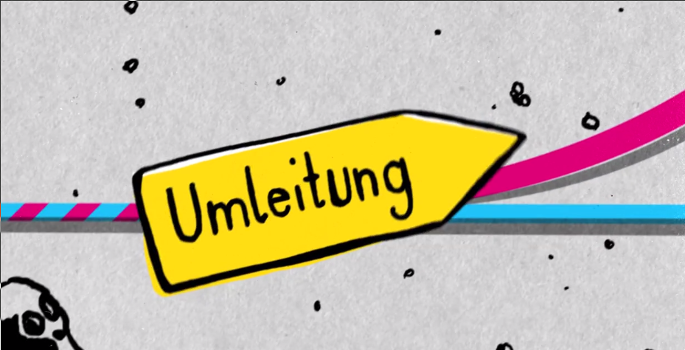
\includegraphics[width=0.9\textwidth]{images/umleitung}
        \vspace{1em}
           Durch die Umleitung des Datenverkehrs müssen sich Betreiber von Freifunk-Knoten um die Störerhaftung also keine Gedanken machen.
        \vspace{1em}
      \end{column}
    \end{columns}
  \end{frame}

  \begin{frame}{Und wie sieht das in der Praxis aus?}
    \begin{center}
      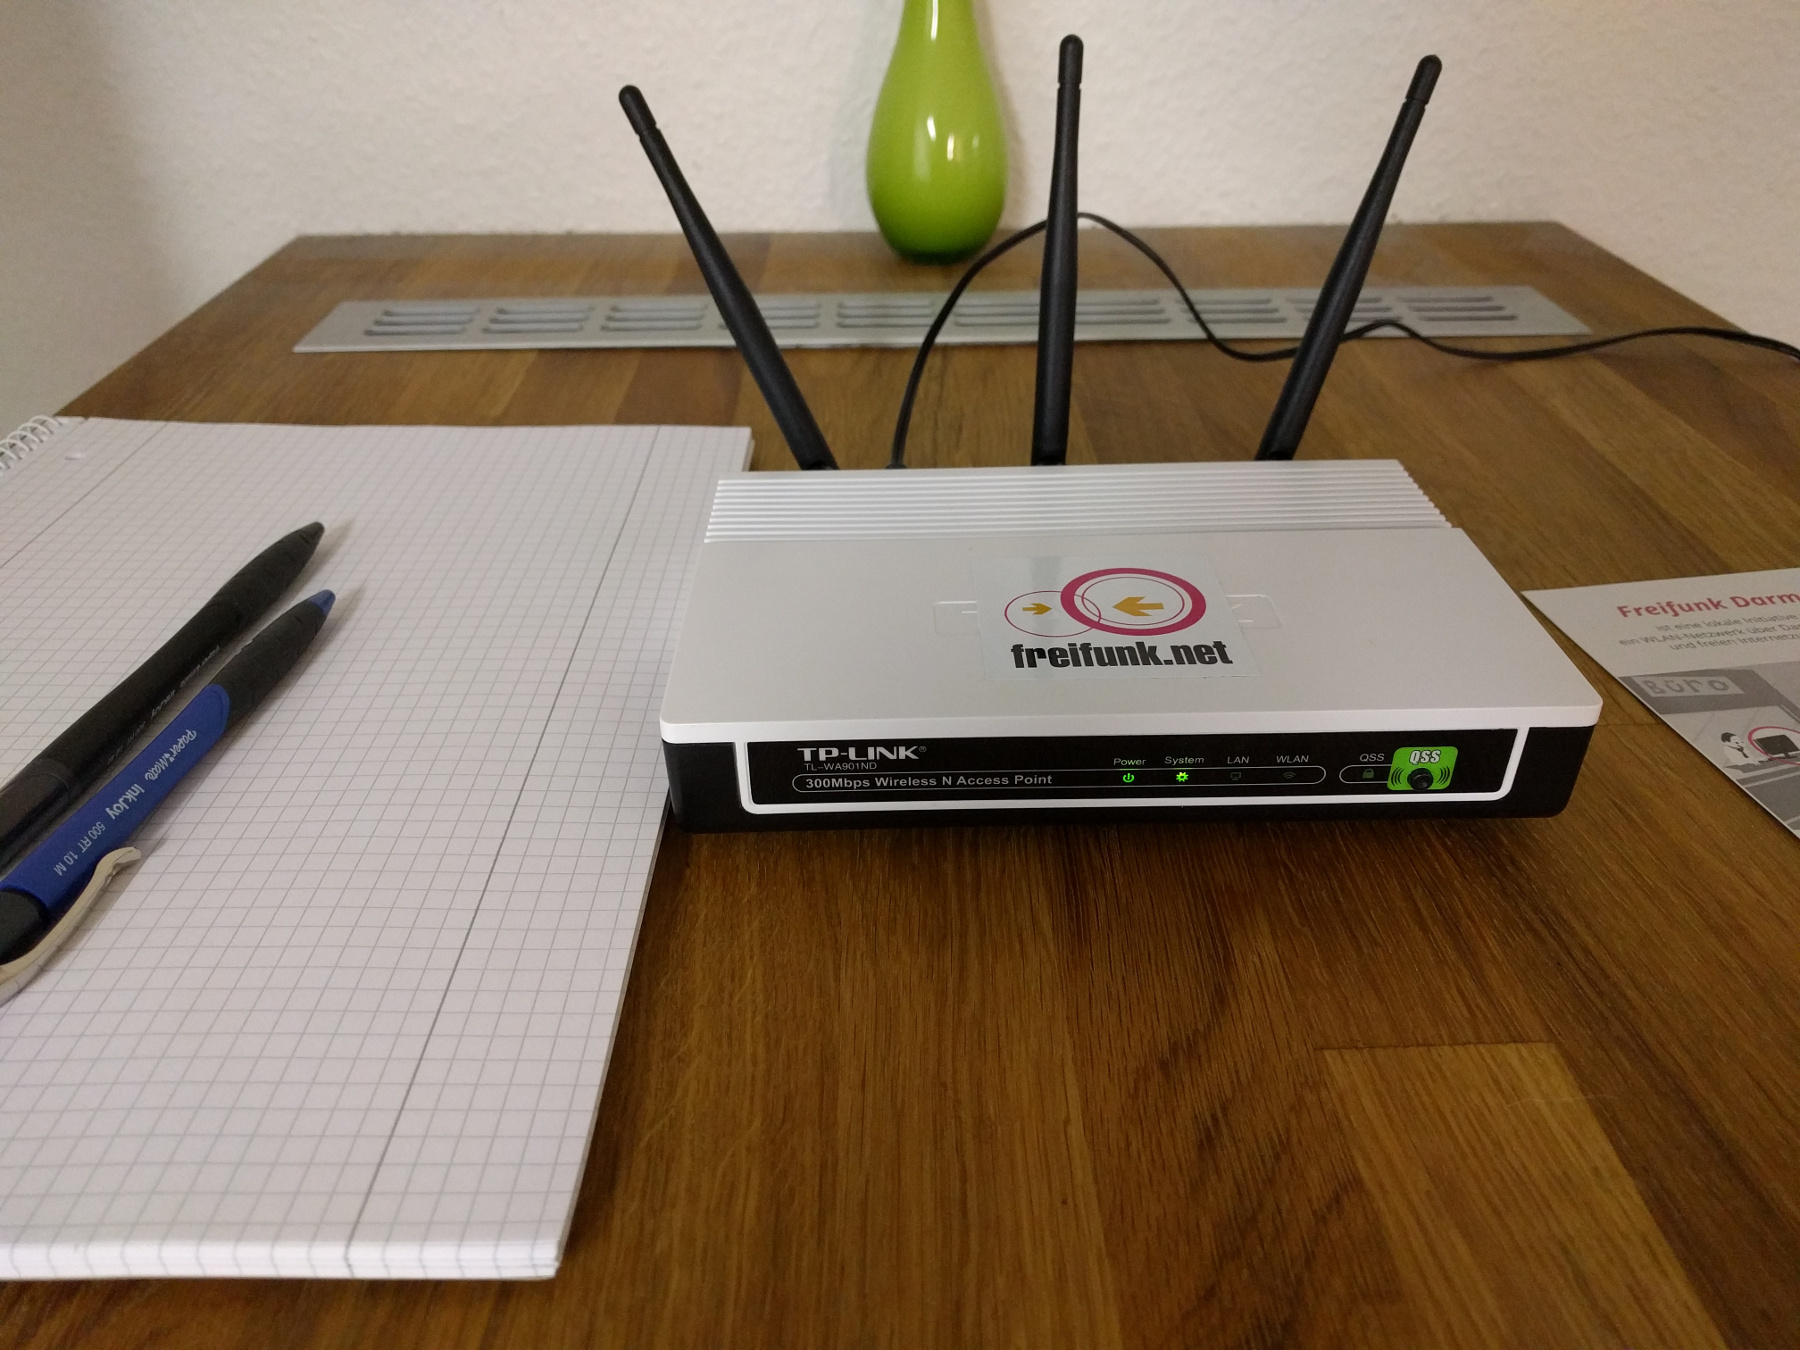
\includegraphics[width=9cm]{images/homerouter}
    \end{center}
  \end{frame}

  \section{Freifunk in der Ortenau}
  \begin{frame}{Freifunk in der Ortenau}
        \begin{itemize}
          \item[\textcolor{freifunkpink}{\Large$\bullet$}] Idee besteht seit 2015, Gegründet im Juni 2016
          \item[\textcolor{freifunkpink}{\Large$\bullet$}] Derzeit ca. \textbf{25 Zugangspunkte} in der Ortenau geschaffen
          \item[\textcolor{freifunkpink}{\Large$\bullet$}] Es besteht eine enge kooperation mit Freifunkern aus Karlsruhe (Technik/Community)
          \item[\textcolor{freifunkpink}{\Large$\bullet$}] Derzeit im Gespräch mit der Stadt Offenburg über Freifunk-Netz in der Innenstadt
        \end{itemize}
  \end{frame}

  \begin{frame}{Freifunk in der Ortenau}
    \begin{center}
        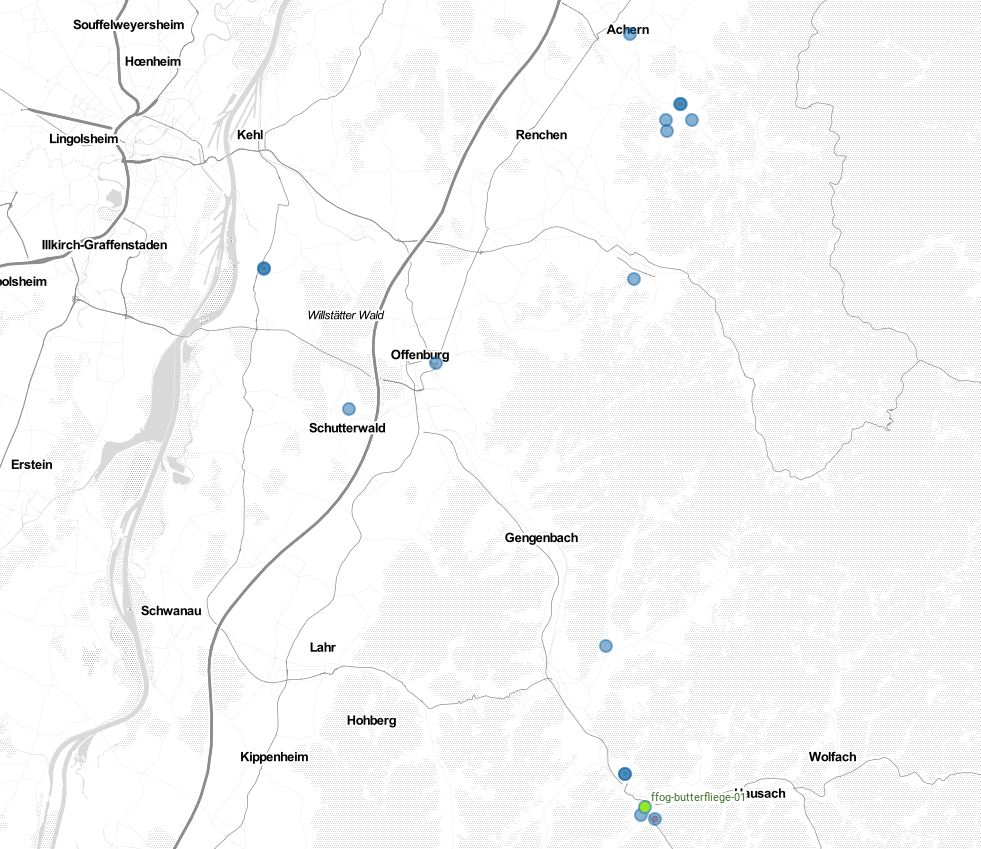
\includegraphics[height=5cm]{images/knotenkarte}\\
        \begin{itemize}
           \item[\textcolor{freifunkpink}{\Large$\bullet$}] Karte mit Zugangspunkten, abrufbar unter: \url{https://ortenau.freifunk.net/karte}
        \end{itemize}
    \end{center}
  \end{frame}

  \begin{frame}{Wie kann ich mitmachen?}
    \begin{columns}[T]
     \begin{column}{5cm}
	\vspace{1em}
        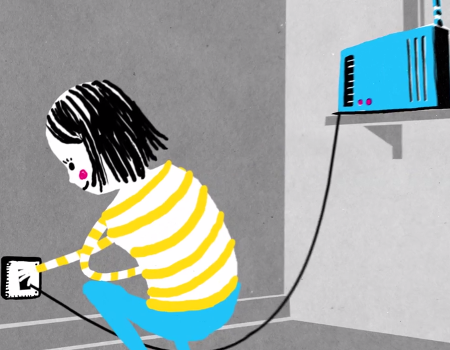
\includegraphics[width=0.9\textwidth]{images/setup}
      \end{column}
      \begin{column}{5cm}
        \begin{itemize}
          \item[\textcolor{freifunkpink}{\Large$\bullet$}] Besorge dir einen \textbf{kompatiblen WLAN-Router}
          \item[\textcolor{freifunkpink}{\Large$\bullet$}] Installiere darauf die \textbf{Freifunk-Software}
          \item[\textcolor{freifunkpink}{\Large$\bullet$}] \textbf{Setze ein paar Einstellungen} wie Knotenname, Aufstellort oder eine Bandbreitenbegrenzung
          \item[\textcolor{freifunkpink}{\Large$\bullet$}] \textbf{Fertig!} Nun bist du Teil des Freifunk-Netzwerkes und ermöglichst allen in der Nähe den Zugriff auf das Internet und auf das Freifunk-Netz
        \end{itemize}
      \end{column}
    \end{columns}
  \end{frame}

  \begin{frame}{Welche Router sind kompatibel?}
    \begin{center}
      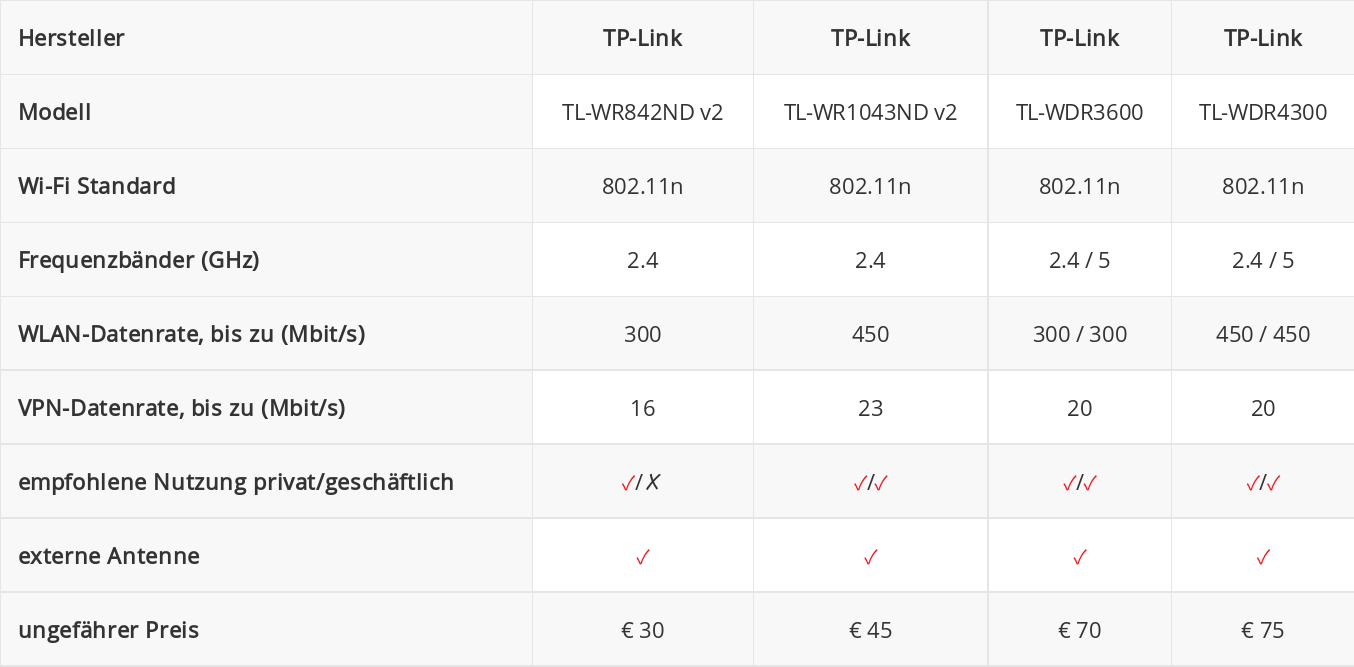
\includegraphics[height=4.85cm]{images/router_recommendation_table}\\
      \vspace{1em}
      Eine Liste mit kompatiblen Routern findest du auf unserer Webseite. Wir können die Router aus der obigen Tabelle empfehlen.
      \vspace{1em}
    \end{center}
  \end{frame}


  \begin{frame}{Wir freuen uns auf Euch!}
    \hspace{1em}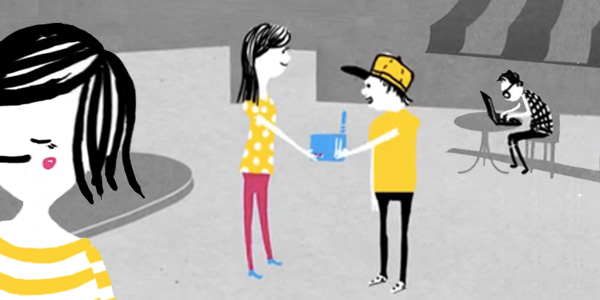
\includegraphics[width=0.6\textwidth]{images/router}
    \begin{itemize}
      \item[\textcolor{freifunkpink}{\Large$\bullet$}] Wir treffen uns jeden 2. und 4. Mittwoch um 20 Uhr in den Räumen des Section 77 e.V.
      \item[\textcolor{freifunkpink}{\Large$\bullet$}] Komme vorbei, wir helfen dir gerne beim Installieren und Einrichten der Software
      \item[\textcolor{freifunkpink}{\Large$\bullet$}] Registriere dich auf unserer Mailingliste
      \item[\textcolor{freifunkpink}{\Large$\bullet$}] Weitere Kontaktmöglichkeiten auf unserer Webseite:\\
      \url{https://ortenau.freifunk.net/kontakt/}
    \end{itemize}
  \end{frame}

  \begin{frame}{Wir freuen uns auf Euch!}
    \begin{center}
      \hspace{1em}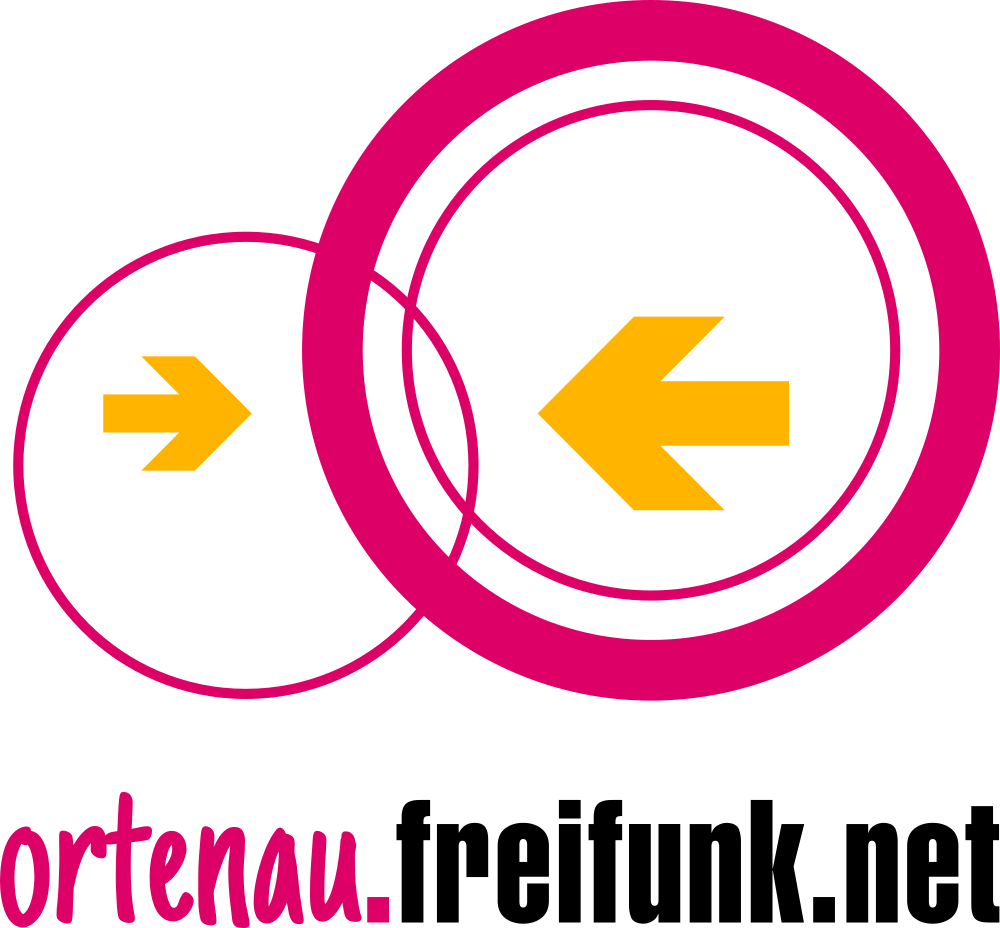
\includegraphics[width=0.35\textwidth]{images/freifunk_ortenau_logo_1000.png}\\
    \end{center}
	\textbf{Vortrag von:}	Jannis Pinter (jannis@pinterjann.is)\\
        \textbf{Webseite:}	\url{https://ortenau.freifunk.net}\\
        \textbf{Präsentation:}	\url{https://ortenau.freifunk.net/files/presentations/\jobname.pdf}\\
        \textbf{Lizenz:}	CC0
  \end{frame}

\end{document}
